\chapter{Methodology}\label{ch:4}

In this chapter, we are first going to introduce our problem at hand -- including an overview of the dataset we are going to be working with, then describe the methodologies of our architecture exploration process and results analysis, and finish with a section about our model training regime.

\section{The system identification task}

We are going to work with data recorded by \cite{antolik} in mouse primary visual cortex, trying to capture the computation of retinal ganglion cells, LGN, and both simple and complex cells of V1.

\begin{itemize}
	
	\item\textbf{Stimuli:} Static images of natural scenes, such as landscapes, animals, or humans, from David Attenborough’s BBC documentary Life of Mammals. The images were presented to sedated mice in 256 luminance steps grayscale and downscaled to 384x208 pixels.
	
	\item\textbf{Recorded response:} The estimated average number of spikes of a neuron in a specific time window after an image stimulus presentation. Recorded by calcium imaging method and further processed by spike extraction algorithm\footnote{The response is actually not a spike count but a variable directly proportional to it.}. In our case, a whole population of tens of neurons within a small region of V1 was simultaneously recorded for each stimulus.
	
\end{itemize}

The fact that we are working with natural stimuli is important. While the function of V1 neurons, especially simple cells, is relatively known for artificial stimuli such as white noise or small contrast lines of various orientations, the computation of complex cells on natural stimuli, containing all sorts of high and low frequency details and cross correlations, is still an open question. This is a direct consequence of the nature of simple and complex cells as intruded in \refsection{ch:1.1.1}. 

Due to the functional organization of mammalian V1, neurons recorded in a local area of visual cortex all have receptive fields within a restricted region of their visual space. Thus, there is no reason to use the entire stimulus image for response modeling. Instead, receptive fields of individual recorded neurons were estimated using a rLN model on the full stimulus and combined to form a region of interest. To account for inaccuracies, this region spanned roughly two times the area of the union of individual neurons’ estimated receptive fields. Lastly, only these regions of interest were cut out of the stimuli pictures, downscaled to 31x31 pixels, and used to form our dataset’s inputs.

\subsection{Dataset}\label{ch:4.1.1}

The dataset consists of three regions, each recorded separately, targeting different neurons, and with an individual set of stimuli. The regions contain 103, 55, and 102 recorded neurons respectively. Each region consists of a training set, with stimuli each presented only once, as well as an explicit validation set (also referred to as the test set), where each stimulus was presented 10, 8, and 12 times respectively and the responses were averaged. The training sets contain 1800, 1260, and 1800 images for the three regions while each validation set is 50 images regardless of region. Regions 1 and 2 were recorded in one animal and region 3 with another.

\begin{table}[h]
    \renewcommand{\arraystretch}{1.0}
    \centering
    \begin{tabular}{l|l|l|l}
        \toprule
        & \textbf{Region 1} & \textbf{Region 2} & \textbf{Region 3} \\ \midrule
        Recorded neurons & 103 & 55 & 102 \\ 
        Training stimuli & 1800 & 1260 & 1800 \\ 
        Training repetitions & 1 & 1 & 1 \\ 
        Validation stimuli & 50 & 50 & 50 \\ 
        Validation repetitions & 10 & 8 & 12 \\ 
        Animal & A & A & B \\ \bottomrule

    \end{tabular}
    \caption[Regions of dataset]{Summary of regions within the dataset.}
    \label{tab:4.1}
    \renewcommand{\arraystretch}{1.0}
\end{table}

The fact that the validation sets are averaged across multiple stimulus presentations while the training set is recorded only once has consequences in terms of the measured responses’ signal to noise ratio. To illustrate this: the average correlation between predicted and measured responses across region 1 neurons, as reported by \cite{antolik}, was between\footnote{Depending on random initialization.} 0.28 and 0.35 on the training set and between 0.41 and 0.52 on the validation set for the same models. Similarly for the other two regions, the performance on their validation sets was substantially higher than for the training sets. 

The stimuli, representing 31x31 pixel 8-bit grayscale images, are stored as float64 numpy arrays of appropriate dimensionality. Inexplicably, the range of pixel values is 0-0.000255 instead of the expected 0-255. For each stimulus, the measured response is a recorded-neurons-wide floating point vector representing variables each proportional to a measured neuron’s spike rate. They are stored as a float64 numpy array of respective dimensionality. The responses have a range of roughly 0-10.

\subsection{Prior works results}\label{ch:4.1.2}

Both \cite{antolik} and \cite{klindt} published results of several models on the \citeauthor{antolik} dataset as part of their papers. Table \ref{tab:4.2} shows a subset of models and their reported validation set correlations that will either be referenced later or we deem relevant for the context they provide.

\begin{table}[ht]
    \renewcommand{\arraystretch}{1.0}
    \centering
    \begin{tabular}{l|l|l|l|l}
        \toprule
        \textbf{Model} & \textbf{1} & \textbf{2} & \textbf{3} & \textbf{Paper} \\ \midrule
        HSM & 0.51 & 0.43 & 0.46 & \citeauthor{antolik} \\ 
        rLN & 0.51 & 0.43 & 0.46 & \citeauthor{antolik} \\ 
        What/Where & 0.51 & 0.43 & 0.46 & \citeauthor{antolik} \\ 
        What/Where: fully-connected readout & 0.51 & 0.43 & 0.46 & \citeauthor{klindt} \\ 
        Linear-nonlinear Poisson (LNP) & 0.51 & 0.43 & 0.46 & \citeauthor{klindt} \\ \bottomrule
    \end{tabular}
    \caption[Performance of prior works.]{Validation set correlation of prior works models on all three dataset’s regions.}
    \label{tab:4.2}
    \renewcommand{\arraystretch}{1.0}
\end{table}

Since much of our analysis is focused on stability of model performance with respect to random initialization, table \ref{tab:4.3} provides validation set correlations of 50th, 10th, and 90th percentiles\footnote{For the rationale refer to \refsection{ch:4.3.1}.} across 100 separate fittings using different initial conditions of the \textit{HSM model}, as reported by \citeauthor{antolik} Regrettably, similar data are not available for \citeauthor{klindt} model or any other of the aforementioned models.

\begin{table}[ht]
    \renewcommand{\arraystretch}{1.0}
    \centering
    \begin{tabular}{l|l|l|l}
        \toprule
        & \textbf{50th} & \textbf{90th} & \textbf{10th} \\ \midrule
        Region 1 & 0.479 & 0.501 & 0.442 \\ 
        Region 2 & 0.412 & 0.435 & 0.382 \\ 
        Region 3 & 0.437 & 0.449 & 0.419 \\ \bottomrule

    \end{tabular}
    \caption[Performance percentiles of HSM model]{Percentiles of validation set correlations of \textit{HSM model} across 100 different random initializations.}
    \label{tab:4.3}
    \renewcommand{\arraystretch}{1.0}
\end{table}

\section{Experiments}\label{ch:4.2.1}

Due to the size of both hyperparameters and especially architecture space, a complete exploration that would cover all possible combinations of a model for our dataset is not possible. It is not feasible even if we assume starting off a preexisting architecture, in our case the \textit{HSM model} by \cite{antolik}, and would only want to explore its close neighborhood -- architecture and hyperparameter wise. 

Instead of trying all combinations, we opted for the following approach. We start with a working model called and call it \textit{baseline}\footnote{The first \textit{baseline} will be a reimplementation of the \textit{HSM model} by \cite{antolik}}. With it as a base, we conduct a set of smaller exhaustive grid search \textit{experiments}, each focused on a small set of hyperparameters or architecture aspects. After analysing these \textit{experiments}, we combine the modifications that worked best and assess the performance of this new \textit{baseline} model. This step is important to verify the additivity of separately tested improvements. If the new \textit{baseline} model candidate performs better than the current one, it becomes the new \textit{baseline}. After that, the cycle repeats with a new set of \textit{experiments}. For future reference, the term \textit{experiment} refers to a single focused grid-search exploration and \textit{experiment instance} to one particular model with a specific set of hyperparameters that is, among others, assessed as part of an experiment.

Contrary to the classical deep learning assumption \citep{2017arXiv170610239W} that modern optimization techniques on real-world datasets should converge to reasonably similar levels of performance and generalization across multiple random initializations, \citeauthor{antolik} described a substantial variance\footnote{Refer to \refsection{ch:4.1.2}.} for different initializations and subsequent training of the same model. To control for this phenomenon, all our \textit{experiment instances} are run multiple times, each time with a different random seed (further referred to as \textit{experiment instance run}). To facilitate repeatability\footnote{It is important to note that TF and thus NDN3 is not entirely deterministic. For more information, refer to: \href{https://github.com/NVIDIA/framework-determinism}{https://github.com/NVIDIA/framework-determinism}.}, consecutive seeds starting at 0 are used.

\begin{figure}[ht]
    \centering
    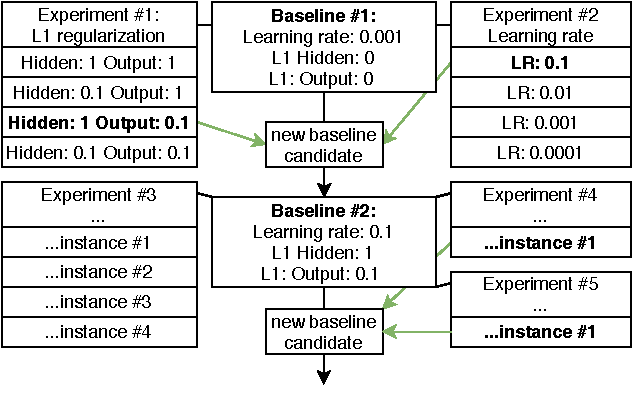
\includegraphics[]{../figures/04_explor_1}
    \caption[Experiments methodology]{Experiments methodology: Bold instances represent better performance than respective \textit{baseline} models. Black lines show what \textit{baseline} model was used for an experiment. Green arrows show improvements of best instances selected to form a new \textit{baseline} candidate.}
    \label{fig:4.1}
\end{figure}

\begin{enumerate}[noitemsep]
    \item \texttt{Assess the performance of a baseline model.}
    \item \texttt{Run a set of experiments, each testing a modification of the\\ baseline model.}
    \begin{enumerate}[nosep]
        \item \texttt{Grid search experiment instances to cover all parameters\\ of the change.}
        \begin{enumerate}[nosep]
            \item \texttt{Execute multiple runs of each experiment instance.}
        \end{enumerate}
    \end{enumerate}
    \item \texttt{Take experiment instances that worked best and performed\\ better than baseline, combine them to a new model.}
    \item \texttt{Verify the new model is better than the old baseline. If it\\ is, make it a new baseline.}
    \item \texttt{Repeat, go to 2.}
\end{enumerate}
\begin{center}
    {The experiment exploration algorithm.}
\end{center}

The same seeds are used across both different \textit{experiments} and different \textit{experiment instances}. Therefore, all other things equal, the \textit{first run} of \textit{instance 1} of \textit{experiment  1} has the same seed as the \textit{first run} of \textit{instance 2} of \textit{experiment 1} or the \textit{first run} of \textit{instance 1} of \textit{experiment 2}. Due to that, runs of the same architecture differing only by hyperparameters that do not influence the number or order of randomly initialized parameters should be initialized with the same values.

Instead of this approach, we could have chosen to use either a fully automated or at least partially computer assisted method to search the model space, for example through evolutionary algorithms \citep{2017arXiv170300548M}, Bayesian optimization \citep{thesis_arnold}, or deep learning based autoML system \citep{2016arXiv161101578Z}. That would, however, go against our goal to test specific modifications to \citeauthor{antolik}’s model and carefully mix it with and compare to elements from traditional DNN toolkit. A comparison between our work and a more automated approach would be an interesting topic for further research but is outside of the scope of this thesis.

\section{Analysis}\label{ch:4.3.1}

As explained in the \refsection{ch:4.2.1}, when assessing two model instances we are not comparing two \textit{runs}, one per each \textit{instance}, but two \textit{distributions of runs}. That complicates analysis as we cannot simply say that \textit{instance A} is better than \textit{instance B} because it achieves a higher performance metric, Pearson’s correlation in our case\footnote{For reasoning refer to \refsection{ch:1.4.2}.}, on the validation set at the end of training. Instead, we have to decide what is the representative sample out of the two distributions of runs to compare. Further, we also have to consider the variance across multiple \textit{runs}, as it represents the stability of the model with respect to random initialization -- an aspect we set out to explore. A model that has slightly better e.g. 90th percentile run but has two times as large variance between runs -- leading to significantly worse 10th percentile, than the baseline model is neither clearly better nor worse, but is noteworthy. 

Thus, with a few exceptions, we report three metrics per \textit{experiment instance}. The median correlation on validation set, 90th and 10th percentiles. We chose to report these to present a clear picture of how big of a spread individual models have depending on random initialization. Together with the higher number of runs per each \textit{experiment instance}, it also makes reasonably sure we do not present random outliers while showcasing the full potential. Unlike variance, percentiles allow for accurate representation of non-symmetrical variances\footnote{E.g. when half of the \textit{runs} have good performance and the other does not train at all. In that case, the 50th and 90th percentiles would be close to each other -- showcasing the potential, and the 10th would be near zero correlation.} and directly show what exact level of performance the model instance is capable of.

It is important to note that each run is not represented by just a single scalar -- its performance at the end of training, but a time series that shows the progress during training. For simplification, we will mostly consider only either the end of training or peak value, however. When relevant, we will draw explicit attention to the speed of convergence or other phenomena apparent only when the whole training in time is considered.

\section{Training regime}\label{ch:4.4}

We opted for a simple static and fully predetermined amount of training epochs. The reason why we did not choose early stopping instead is threefold. First, it is the simpler solution without additional hyperparameters and implementational complexity. Second, we only have limited data that is already explicitly divided into train and validation sets. Splitting either to form a test set to evaluate early stopping on might compromise either training or validation due to insufficient data. Third, due to the size of the validation set, we evaluate it fully throughout the training process, capturing all relevant performance metrics\footnote{Refer to \refsection{ch:3.1.1}.}. Thanks to that, we always have the full information about the model’s peak performance on the validation set, even if we overfit after achieving it. This leaves computational efficiency as the only benefit of early stopping, which in our opinion did not outweigh the negatives\footnote{\cite{klindt} report using early stopping with a training set split of 80/20, refer to \refsection{ch:2.2}}.

Based on early tests, we chose to train \textit{experiments} for 5 000 epochs and \textit{baseline} models for 35 000 epochs. This proved to be more than enough for experiment instances to show potential -- if there was any, and for \textit{baseline} models to achieve peak performance and -- in case they were susceptible to it -- overfit, with plenty headroom especially for later models. 

In regards to the number of \textit{runs} per model \textit{instance}, we have chosen 10 runs for experiment instances and 25 runs for baseline model instances to balance computational resources and statistical significance of the results. The effect of potentially higher numbers of runs on one of the least stable \textit{baseline} models can be seen on figure \ref{fig:4.2}.

Unless explicitly mentioned, all of our experiments are evaluated only on region 1. Region 1 was chosen due to being the largest, highest performing, and least stable of the three regions -- as reported by \citeauthor{antolik} In \refsection{ch:5.3.2} we evaluate the main architectures explored and fine-tuned on region 1 on regions 2 and 3 as well.

\begin{figure}[H]
    \centering
    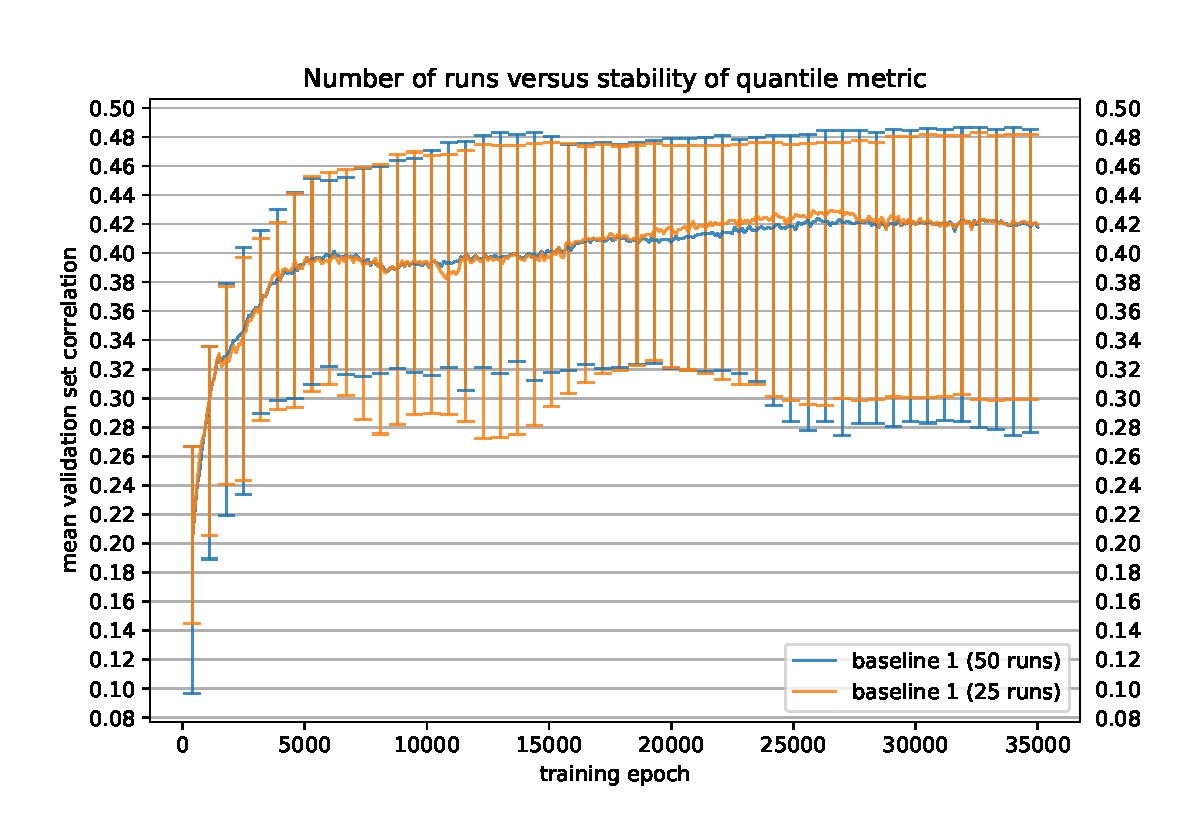
\includegraphics[width=0.99\textwidth]{../figures/04_runs_number}
    \caption[Impact of 25 vs 50 runs]{Illustrates the difference between running the least stable \textit{baseline} model 25 and 50 times. The line represents median run, top and bottom error bars 90th and 10th percentile runs.}
    \label{fig:4.2}
\end{figure}
